\documentclass[twocolumn]{article}
\usepackage{graphicx}
\usepackage{caption}
\usepackage{subfigure}
\usepackage[pdfborder={0 0 0},plainpages=false]{hyperref}
\usepackage{url}
\usepackage{tikz}
\usetikzlibrary{shapes,arrows,automata}

\title{Bachelor thesis plan of approach}
\author{Chiel de Roest\\4036832 \and Harmjan Treep\\4011724}
\date{}

\newcommand{\protospace}{\textit{proto}SPACE }

\begin{document}

\maketitle

\begin{figure}
	\centering
	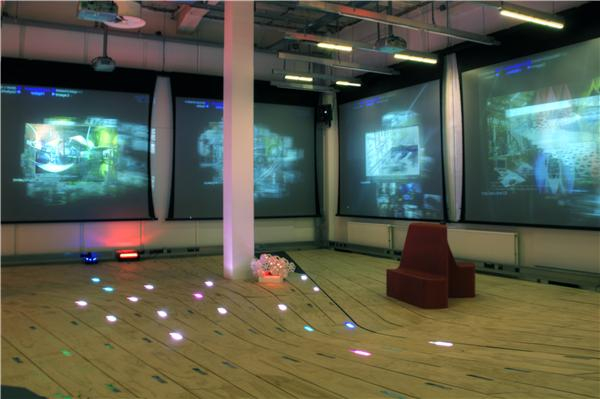
\includegraphics[width=\columnwidth]{protospace}
	\caption{The \protospace 3.0 room}
	\label{fig:protospace}
\end{figure}

\section{Introduction}
	The hyperbody research group (\url{http://www.hyperbody.bk.tudelft.nl/}) in faculty of Architecture has the goal to
	\begin{quote}
		explore techniques and methods for designing and building of non-standard, virtual and interactive architectures.
	\end{quote}
	A room in the faculty of Architecture has been equipped with a floor with nodes in it.
	Each of these nodes has a RGB LED and a pressure sensor.
	This room is called \protospace 3.0 as seen in Figure \ref{fig:protospace}.
	
	The faculty of EWI and Industrial Design also play a role in this.
	The Embedded Systems group of EWI plays a role in the hyperbody project by developing the hardware and software for this room.
	We are doing our bachelor project in this group by developing tools to use for debugging the floor.
	
	In this document we will describe what the project entails and how we plan to approach this project.
	
	The floor in \protospace 3.0 is implemented as seen in Figure \ref{fig:network}.
	Every node (tile) can talk to its neighbours via an UART connection, the black arrows in Figure \ref{fig:network}.
	But there is also a CAN bus that all nodes can talk over, the red line in Figure \ref{fig:network}.
	
	\begin{figure}[t]
		\centering
		\tikzstyle{square}=[rectangle,thick,minimum size=0.5cm,draw=blue!80,fill=blue!20]
		\begin{tikzpicture}[auto, outer sep=3pt, node distance=2cm,>=latex']
			\node [square] (1) {Node 1};
			\node [square] (2) [right of=1] {Node 2};
			\node [square] (3) [right of=2]{Node 3};
			\node [square] (4) [below of=1]{Node 4};
			\node [square] (5) [right of=4]{Node 5};
			\node [square] (6) [right of=5]{Node 6};
			\node [square] (7) [below of=4]{Node 7};
			\node [square] (8) [right of=7]{Node 8};
			\node [square] (9) [right of=8]{Node 9};
			
			\draw [<->,thick] (1) --  node {} (2) ;
			\draw [<->,thick] (2) --  node {} (3) ;
			\draw [<->,thick] (1) --  node {} (4) ;
			\draw [<->,thick] (2) --  node {} (5) ;
			\draw [<->,thick] (3) --  node {} (6) ;
			\draw [<->,thick] (4) --  node {} (5) ;
			\draw [<->,thick] (5) --  node {} (6) ;
			\draw [<->,thick] (4) --  node {} (7) ;
			\draw [<->,thick] (5) --  node {} (8) ;
			\draw [<->,thick] (6) --  node {} (9) ;
			\draw [<->,thick] (7) --  node {} (8) ;
			\draw [<->,thick] (8) --  node {} (9) ;
			
			\path[red,thick] (7) edge [bend left] node {} (4)
			      (4) edge [bend left] node {} (1)
			      (1) edge [bend left] node {} (2)
			      (2) edge [bend right] node {} (5)
			      (5) edge [bend right] node {} (8)
			      (8) edge [bend right] node {} (9)
			      (9) edge [bend left] node {} (6)
			      (6) edge [bend left] node {} (3);
		\end{tikzpicture}
		\caption{A sensor node network with a CAN bus}
		\label{fig:network}
	\end{figure}

\section{Assignment}
	Our assignment is to develop tools for development of code for the network.
	We interpreted this as the following list tasks:
	\begin{itemize}
		\item Flash an image on a node over the CAN bus;
		\item Download code into an already running eLua VM;
		\item Create a debugging environment for eLua, such as starting, stopping or inspecting a variable on a node;
		\item A command to load all nodes in the network to a known state.
	\end{itemize}
	We will try to execute these tasks in this order.
	
	We will implement this in the hardware used in the \protospace 3.0 room, LPCXpresso board with the in house developed LPCXpresso shield attached.

\section{Approach}
	Our goals are very broad and daunting, we also are not fully aware of our capabilities in developing embedded software and therefore we have decided to adopt a agile development process.
	We will meet with our supervisor S. Dulman every week on Monday and in that meeting we will discuss progress and problems.
	We will setup a set of goals for the next week.
	Every day we will have a meeting with just the two of us discussing the goals for that day.
	
	In the beginning of the project we will familiarize ourselves with the hardware platform and the tools used for developing on that platform.
	The results of this will be discussed in our orientation report.

\end{document}
